\documentclass[twoside,a4,12p]{report} %,draft,openright]

\usepackage{epsf,graphicx}
\usepackage{latexsym,amssymb}
\usepackage{setspace,cite}
\usepackage{array}
\usepackage{amstext}
\usepackage{amsmath}
\usepackage{fancyhdr}
\usepackage{float}
\usepackage[LGRgreek]{mathastext}
\usepackage{lipsum}
\usepackage{multirow}
\usepackage{subfigure}
\usepackage{url}
\usepackage{varwidth}
\usepackage{booktabs}
\usepackage[table]{xcolor}
\usepackage{tabularx}
\usepackage{arydshln}
\usepackage{datatool}
\usepackage{courier}
\usepackage{lscape}
\usepackage{pdflscape}
\usepackage{siunitx}
\usepackage{bbding}
\usepackage{pifont}
\usepackage{wasysym}
\usepackage{amssymb}


% for margins left, right top bottom
\usepackage{anysize}
\marginsize{4cm}{2.5cm}{4cm}{4cm}

%\usepackage{draft} %draft option - doesn't put full figures in -
            % useful when editing

%does the headers on the pages - keep in
\usepackage{fancyhdr}


%omitting any of these makes the thesis compile without the omitted
%chapter - good for editing single chapters.
\includeonly{header,intro,background,appendix}
\usepackage{acro}
\DeclareAcronym{dc}{
  short = DC,
  long  = Dice Coefficient
}

\DeclareAcronym{sf}{
  short = DC,
  long  = Dice Coefficient
}

\begin{document}
\newpage

%Puts page numbering of preamble in roman and of main body of thesis in
%arabic. Also defines how chapters and sections are made
\pagenumbering{arabic}
\setcounter{page}{1} \pagestyle{fancy}
\renewcommand{\chaptermark}[1]{\markboth{\chaptername%
\ \thechapter:\,\ #1}{}}
\renewcommand{\sectionmark}[1]{\markright{\thesection\,\ #1}}

%DEFINES TITLE PAGE, and contains abstract, acknowledgements, etc.

%%%%%%%%%%%%%%%%%%%%%%%%%%%%%%%%%%%%%%%%%%%%%%%%%%%%%%%%%%%%%%%%%%%%%%%%%%%
% This is a sample header for a sample dissertation. Fill in the name,
% and the other information. LaTeX will work out the table of
% content, the list of figures and of tables for you.
%%%%%%%%%%%%%%%%%%%%%%%%%%%%%%%%%%%%%%%%%%%%%%%%%%%%%%%%%%%%%%%%%%%%%%%%%%%

\newpage
\thispagestyle{empty}

% ******* Title page *******
% **************************

\vspace*{2cm}
\begin{center}
{\Large\bf Optimized Waypoints selection for UAV maximum area coverage\\} \vspace{2cm} {\large
Mark Bastourous\\
\vspace{2cm}
LE2I - Laboratoire Electronique, Informatique et Image \\
Universite Bourgogne Franche-Comte}\\


\end{center}

\vspace{7cm}
\begin{center}
{\large A Thesis Submitted for the Degree of \\MSc in Computer Vision and Robotics 
(MSCV) \\\vspace{0.3cm} $\cdot$ 2016
$\cdot$}
\end{center}
\singlespacing


%ABSTRACT
\begin{abstract}
The abstract will go here....

\vspace*{5cm}



\begin{center}
\begin{quote}
\it Research is what I'm doing when I don't know what I'm
doing.\,\ldots
\end{quote}
\end{center}
\hfill{\small Werner von Braun}

\end{abstract}

\doublespacing

%\pagestyle{empty}
\pagenumbering{roman}
\setcounter{page}{1} \pagestyle{plain}


\tableofcontents

\listoffigures
\listoftables

\chapter*{Acknowledgments}

\addcontentsline{toc}{chapter}
         {\protect\numberline{Acknowledgments\hspace{-96pt}}}
To be mentioned David Fofi , Morel , Strubl
,Family : Bro , Ma , Fa .

\pagestyle{fancy}


\newpage

%sets up headers for lefthand and righthand pages. To alter, edit
%these lines and the chaptermark/sectionmark lines above
\addtolength{\headheight}{3pt} \fancyhead{}
\fancyhead[LE]{\sl\leftmark} \fancyhead[LO,RE]{\rm\thepage}
\fancyhead[RO]{\sl\rightmark} \fancyfoot[C,L,E]{}
\pagenumbering{arabic}

%\singlespacing
%\doublespacing
\onehalfspacing
\chapter{Introduction} \label{chap:intro}

\iffalse
\section{Preparing your dissertation} \label{sect:thefirst}

You are strongly encouraged to use the Latex templates provided.

\subsection{Paper}
The manuscript should be in A4 size, and the printed paper should
be of at least 70 gsm.

\subsection{Font and margins}
Thesis should be printed on both sides of the paper. Use no less
than 1.5 spacing, with quotations and notes single-spaced.
Regarding \textbf{Character size}, not less than 2.0mm for
capitals and 1.5mm for x-height (the height of a lower-case x). Us
a serif font (i.e. Times) between 10 and 12 points. Use consistent
and clear fonts through all the document.

The text layout should be approximately as follows:

\begin{itemize}
    \item $4cm$ binding margin
    \item $2cm$ head margin (top of page)
    \item $2.5cm$ fore-edge margin
    \item $4cm$ tail margin (bottom of page)
\end{itemize}

\fi




% \section{Title Page}

% \iffalse
% The title page should contain the title of thesis, authors name,
% and at the foot of the page: the name of degree,  Your University,
% and the year of presentation. Something like this:
% \fi

% \vspace*{1cm}
% \begin{center}
% {\Large\bf Optimized Waypoints selection for UAV maximum area coverage\\} \vspace{2cm} {\large
% Mark Bastourous\\
% \vspace{1cm}
% Laboratoire d'Electronique,Informatique et Image \\
% Universite De Bourgogne}

% \end{center}



% \vspace{2cm}
% \begin{center}
% {\large A Thesis Submitted for the Degree of MSc Computer vision and Robotics Univesite De Bourgogne\\ \vspace{0.3cm} $\cdot$ 2016 $\cdot$}
% \end{center}

% \iffalse
% \subsection{References}
% You can reference other authors by using the $cite command$
% \cite{Pokorski:1998hr}. You are encouraged to use bib files and
% let bibtex do the job for you.
% \fi

\section{INTRODUCTION}

Aerial robots have grown great attention in the last decades due to its capabilities in solving many problems in many domains. They are still under study, investigation and development because of the several constrains and challenges that are in software and hardware of its construction on  many levels and layers. 

Some of the software challenges are state estimation, control, decision making, mapping, and path planning. Some of the hardware challenges are the weight/load ratio, power source, sensors, etc. 

There are various applications that practically make use of unmanned aerial vehicles (UAV) and many more are still under study and development in the research labs and institutes. These applications are covering many fields of interest in both civilian and military purposes. Some of these practical applications are search and rescue, inspections, surveillance, photography, agricultural terrain mapping, mineral exploration, etc. Some prospective applications like medical cargo delivery because it will not rely on the normal road maps if they exist, or traffic constrains that.

There are many types of UAVs categorized based on the geometry and designs like fixed wing, flapping wing, and rotor crafts, mentioned in more details in \cite{UAV_general}. 

\begin{figure}[!htb]
\minipage{0.80\textwidth}
  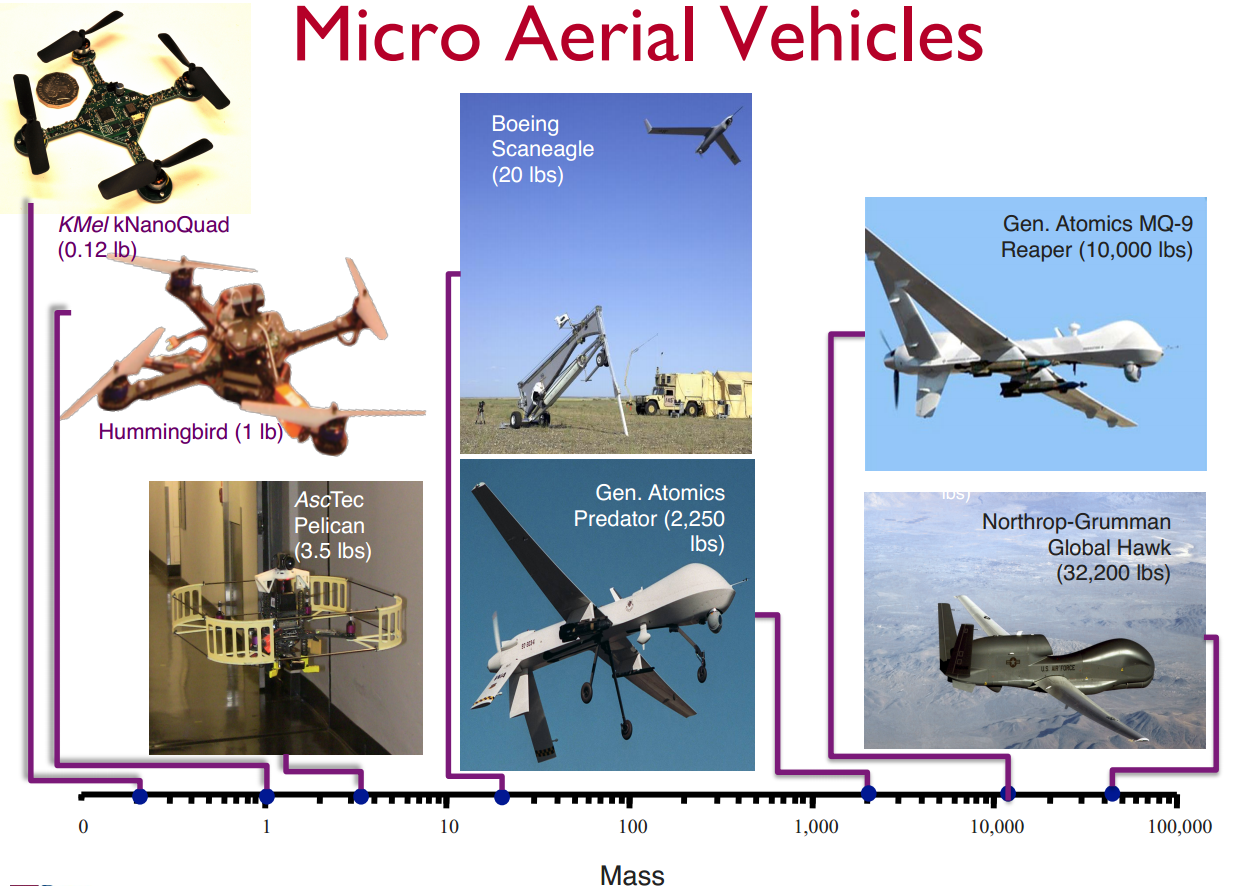
\includegraphics[width=\linewidth]{figures/Micro_aerial.png}
  \caption{Micro aerial vehicle}\label{fig:micro_aerial} \cite{Ardrone2}
  \endminipage\hfill
\end{figure}

The figure \ref{fig:micro_aerial}  shows some of the current UAVs. From cheap and small toys that you can be bought anywhere as the RC planes, toy quadcopter, to big military projects such as the Global Hawk. 

UAVs have recently found decline in their cost especially the quadcopters. In this thesis during the practical implementation part, quadcopters as one type of the rotor crafts will be used. The quadcopter used is Ar.drone 2.0 from the french company parrot. It is offshelf drone that can be found in market with comparable cheap price in range of 300 euros depending on the extras. It has been used several times in research labs and studied in \cite{Ardrone1},\cite{Ardrone2},etc.

There are many advantages that makes quadcopter as specific type of UAVs, suitable for both indoor and outdoor applications. It takes off vertically, do not need a runway, hover in its place, comparably light weight, and small in size.

For simulation V-REP with a model of quadcopter available was used. Some modification in this model was introduced to cope with the problem being solved and will be discussed later in more details. In both the practical work and simulation, ROS packages were used, tuned and implemented to control the quadcopter.

% There was no embedded systems work done and offshelf usage of the drone was utilized.

Some of the previously mentioned applications require area coverage of outdoor or indoor mapping. Coverage path planning is an active research topic as sub division of the general path planning problem that is studied by robotics domain for several decades till our day. It has been applied on many platforms in many areas where these platforms work. Normally the area to be covered is not a regular one. Most of the literature review that come to the awareness to the author of this thesis are concerned with uniform areas and prior map with static or dynamic obstacles in it. Platforms here means the mobile robots like autonomous underwater vehicles(AUV), unmanned aerial vehicle(UAV), or ground vehicles. 

% Aerial robots is still under study, investigation and development because of the many constrains and challenges that are in software and hardware of its construction on  many levels and layers. 

Prior information about the environment is assumed to be given in the form of a rough map for the area required to be covered. For this work, we model the set of coverage problems as arc routing problems. Although these routing problems are generally NP-hard, our approach aims for optimal solutions through the use of low-complexity algorithms in a branch-and-bound framework when time permits and approximations when time restrictions apply.


The final objective of this thesis research is to design a global optimization scheme allowing a cameras network to be self organized or to plan single trajectory of a flying robot equipped with a camera, according to fixed priority and constraints, in order to ensure a full coverage of a given scene. Applicable solution for both indoor and outdoor with ensuring coverage of the terrain while minimizing path repetition. Then building a mosaicking of the area covered and compare it with the original scene.


% %\textcolor{davidS}
% {The main problem of UAVs is the autonomy of fly, because of the battery run-time. This short time action restrained the possibility to use a set of UAVs and the work cooperation for a long time surveillance if there is no much UAVs available at the moment}. One smarter possibility is to create a monitoring path with several UAVs which  %\textcolor{davidS}
% {alternately automatically relays when the battery is low.} 
% During the navigation of the UAV's path, it is possible to get the image of the area to survey and build the mosaic of the area. 
% This paper will focus on finding the best waypoints for the UAV to pass through, to reduce the computation usually done in the path planning and coverage process. In order to find a good path to cover most of the area the essential point is to propose the best waypoints. %Finding the waypoint can be reduced to the problem of finding the best coverage.

% ensures complete coverage of the terrain while minimizing path repetition indoor gps denied  slam methods were used to localize and navigate the UAV using the visual 

In the next subsection the objectives of this thesis will be discussed.

\subsection{Objectives}
\begin{itemize}

\item Study coverage path planning problem, implement the suitable one.
\item Test and validate the path planning in both simulation and real world with practical hardware.
\item Construct a final mosaicked scene after the UAV acquire images.

\end{itemize}

\subsection{Thesis Organization}

\chapter{Background} \label{chap:background}

% Boustrophedon cell decomposition based coverage method 
% not Boustrophedon area coverage from right to left and from left to right in alternate lines.
% veer the uav from the desired path

The merit of this thesis in the coverage path planning context is splitting and decoupling the process of the coverage problem. The process will consist of: finding the proper pose and orientation of camera views that maintain area coverage, then apply path planning techniques to traverse these poses. So that the first part can be used as a solution by itself with positioning cameras in the obtained positions. The second merit is minimizing the overlapping paths and implementing the path planning taking into account the footprint of the robot and the camera, not relying on the assumption of robot representation as a point. % here the footprint of the camera only not the robot too 

\section{Related Work in path planning}
\subsection{Coverage Path Planning}
There are two main surveys that this literature review is relying on in picking and comparing the path planning technique to be further implemented and tested on the quadcopter. These surveys are; a survey on coverage path planning for robotics \cite{CPP2}, and coverage for robotics survey of recent results\cite{CPP1}.

There are a lot of other work extensively explored from many research areas beside path planning like computer vision, and graph theory. The problem can be studied from many sides like mapping, searching, patrolling, and applications. We focus here about the path planning and area coverage problems with slightly different approach than the common one. we take into consideration the footprint of the camera and one of the goals is to reduce the number of waypoints with maximum area coverage. Full area coverage in terms of 100\% is not the constraint.

In the literature generally there is always a navigation pattern to pass through the whole space; the robot need to cover. This pattern is done after decomposing the map into either regular cells or irregular ones like Voronoi. These methods can be categorized as heuristic and approximate, partial-approximate and exact cellular decompositions as discussed in \cite{CPP1}.

Coverage algorithms can be classified as heuristic or complete depending on whether or not they provably guarantee complete coverage of the free space. At the same time, they can be classified as online or offline. Offline algorithms rely only on the stationary information, and the environment is assumed to be known. Usually online algorithms are needed if some kind of adaptivity to the environment is required. Online algorithms usually utilize real-time sensor measurements. Thus, these algorithms can also be called sensor-based coverage algorithms.

The heuristic approach that is based on random path which is like the one equipped in some lawn mower and vacuum cleaner robots as mentioned in \cite{CPP1} can not be considered for aerial robots applications. 
Coverage algorithms can rely on cellular decomposition with many techniques that an extensive comparison was given in \cite{CPP2}; then an ox plowing motions is used like the example in planning algorithm book \cite{planningBook}. As the approach used in this thesis will not rely on map decomposition, further investigation can be found in the cited papers and book. \textcolor{red}{ If not decomposition how to say grid decomposition } 


\textcolor{red}{These algorithm can result in redundant coverage.}

Other approaches like  Artificial Potential Fields (APF), graph algorithms and neural networks can be used instead of the map decomposition. \textcolor{red}{||||||}




\subsection{Coverage Path Planning for UAVs}
There are various ways to obtain the path planning and optimize them.
CPP problem is a sub-field of path planning and well studied for ground vehicles like cases in \cite{CPP1,CPP2,path_planning_UGV}.

\textbf{CPP for UAV in general} 

In operations research, the CPP problem represent the environment as a graph, and using algorithms such as the traveling salesman(TSP) or postman problems to generate optimal solutions. In the graph representation, locations in the environment is represented as nodes in the graph and the paths between the locations are the edges. Each edge has a cost assigned to it where the cost can represent measurements such as distance(Euclidean,Mahalanobis,etc) between locations, terrain traversability, travel time or a combination of several metrics. These edges can be constrained or unconstrained with directions. More precisely undirected , directed graphs.

Voronoi diagram is also another possible solution as developed in \cite{voronoi_UAV} for decomposing the desired area and find the feasible solution from the starting point to the goal point through two step path planning algorithm, but it doesn't take into consideration the repetition rate constraint or full area coverage. For these reasons considering the solution used for arc routing problem is most beneficial.

TSP considered one problem of a large class of problems known as combinatorial problems and introduced in UAV path planning for several purposes like refueling depots in \cite{TSP_UAV}, multiple UAV cooperative reconnaissance in \cite{TSP_UAV_Multi}. This is a non-deterministic polynomial-time hard (NP hard) problem, that is sub-optimally solvable by many approaches as found in various research fields \cite{TSP_NPHARD}. Evolutionary approaches specifically  will be considered in this thesis.  

\subsubsection*{Evolutionary algorithms}

% \textbf{In this thesis considering one UAV operation to solve the CPP problem using GA as global path planning followed by local path planning solution.} 

Evolutionary Algorithms(EA) as sub branch of meta-heuristic optimization algorithms, imitates the biological process of evolution in nature. There are various algorithms that are branched from it like Ant colony optimization (ACO), particle swarm optimization (PSO),Genetic Algorithm GA and many more which can be studied from \cite{Evo_Book1,Evo_Book2}. GA uses techniques of inheritances, mutations, selections and crossovers of chromosomes over several generations of possible solutions to find convergence to the most optimized solution. Explanation in the next chart is the general abstract view of GA, more details will be explained in the methodology chapters.

\tikzset{
  frame/.style={
    rectangle, draw, 
    text width=6em, text centered,
    minimum height=4em,drop shadow,fill=lime!40,
    rounded corners,
  },
  line/.style={
    draw, -latex',rounded corners=3mm,
  }
}

\begin{tikzpicture}[font=\small\sffamily\bfseries,very thick,node distance = 4cm]
\node [frame] (pop) {Population};
\node [above=2cm, left of=pop] (init) {Initialisation};
\node [below=2cm, left of=pop] (term) {Termination};
\node [frame, above=2cm, right of=pop] (parents)  {Parents};
\node [frame, below=2cm, right of=pop] (off)  {Offspring};

\path [line] (parents)
 -- node[right,align=left,pos=.5] {Cross-Over\\[3mm]Mutation}
 (off);
\path [line] (init) |- (pop.170);
\path [line] (pop.190) -| (term);
%tournament 
\path [line] (off) -| node[below,pos=.25, align=center] {Survivor\\ selection}(pop);
\path [line] (pop) |- node[above,pos=.75, align=center] {Parents\\ selection}(parents);
\end{tikzpicture}

\subsection{Hybrid Algorithms for path planning}

\textbf{A two-level approach to collision-free navigation, using
artificial potential fields on the local lower solution planning, and GA solution to waypoints optimization problem represented as TSP for global higher layer planning}. 

then point-to-point motion planning problem, where the vehicle task is to navigate from a pre-specified initial point in the workspace to a pre-specified destination goal point.

\section{Waypoints Selection}

Finding the waypoints to have the best coverage of the area is close to the problem of positioning cameras or sensors to cover an area efficiently. Sensor positioning problem has been investigated since a few decades, mainly for video surveillance \cite{c1}. Without any additional constraint, this problem is NP-Hard as stated in \cite{c1,c2,c3,c4,c5} for the Watchman Route Problem (which is very similar to the optimal positioning waypoint for UAV path). Two non-optimal solutions have been proposed. The first one is based on Art Gallery Problem (AGP) \cite{c2,c3} and the second one is based on the Wireless Sensors Networks \cite{c6,c7,c8,c9} trying to find the best position to design an efficient network which can collect data with any kind of sensors. 

% do you mean here the the sensor pose is the most adequate solution

However, the solution proposed to the problem addressed the coverage problem but linked with additional and specific constraints, which are out of our scope. 
% like basic room without obstacles or focus on selection among the different possible sensor poses, which is the most adequate solutions. 
% This will become finding a solution among a set of more efficient subset of solutions, not a problem of finding a solution
%This will not become a problem of finding a position but to select among the set of more efficient subset of solutions. %or select the position sensor in the set of possible and restrained position
 %\cite{c7}.
 
 One of the algorithm used is the Particle Swarm Optimization (PSO) as detailed in \cite{c10,c11}. Zhou \textit{et al.} \cite{c10}, some experimental results are provided and one solution running in real time is proposed. However, the scene used in these experiments is rather small and many cameras are employed to fully cover it.  On the other hand, \cite{c11} uses a cost function but the cost function is not only focused on the position for surveillance and coverage, but also handling resolution and lighting, which affect the final solution by not covering the under illuminated areas.Reddy \textit{et al}. \cite{c11} also introduced the concept of “acceptable response”, allowing non-optimal/sub-optimal solutions. If the coverage score is higher than a given threshold, the solution is accepted and not locked by the research of an optimal solution. 
% Inspired by \cite{c10,c11}, extending the method for UAV waypoints positioning and path planning in more complex environments (basic room, big room, non-square shape).
 
 \section{UAV Localization} \label{localization_Back}
 
UAV localization problem is the challenge of finding the pose in terms of position and orientation of the aerial robot with reference frame. This reference frame can be with the initial point the robot is launched from, or a point in the map. There are two main categories for localizing the robot; either indoor or outdoor. For outdoor, GPS based navigation system is often used to determine the UAV’s absolute position. Also equipped with inertial measurement unit (IMU), UAV's orientation and acceleration can be estimated. State estimation of the UAV is obtained by coupling the previous obtained data with the UAV's mathematical model. This information is essential for autonomous navigation and of significant importance to aid the pilot to achieve smoother navigation. \textbf{Unlike ground vehicles, just holding the robot's pose requires values to withstand its place , giving order continuously to the robot   This is particularly the case for an aerial vehicle - while for ground-based vehicles not moving typically is a trivial task, this is not the case for a flying robot. Holding a position in the air requires constantly counteracting minor randomly induced movements, which in turn requires a method to detect these movements.}.
While for indoor localization challenge employing the IMU data can provide relative location, over time small errors will keep accumulating and drift will happen and affect the localization. Additional information about global positioning should be available to recover for this drift using means of filtering and sensor fusion \textbf{CITE} 

 This method will not be feasible when flying indoors where there is no reliable or cheaply available GPS modules available - alternative localization methods are required. For these reasons a solution  relying only on the UAV's sensors, using external tracking devices or external fiducial markers tracked by onboard camera. \textbf{CITE} 
 

An example of the available external tracking device are motion capture cameras that allow the robot to measure its position with very high precision and accuracy as in \cite{michael2010grasp}. Reflective markers like retroreflective dots attached to the robot, the cameras can estimate the position of each reflective marker and these cameras can do it at split second timing exceeding speeds of 100-200 times a second. This system will not be used as it requires setup up of several cameras which cost dozens of thousands of euros. The other external solution provided for example in  \cite{meier2012pixhawk} using external markers and detected using onboard camera. This solution could have been considered, but it is not the chosen one to be implemented in this thesis. 
 
 
 There are wide range of sensors can be equipped on the UAV to be help its localization like laser range scanner, monocular camera, stereo camera, RGB-D sensor, or ultrasonic range sensors. The usage of monocular camera is chosen to be the solution for this thesis. They provide competitive advantages; as they are cheap, energy-efficient, small and light. \textbf{CITE} Simultaneous localization and mapping (SLAM) can be achieved by combining visual pose estimates from the monocular camera  with additional sensor measurements available like the implementation of Tardif et al. in \cite{tardif2008monocular}. The tool developed by the computer vision group in Technical University of Munich as mentioned in the papers \cite{engel14ras,engel12iros}, is utilized on an AR.Drone 2.0 available in the lab with minor modification and plugin suitable to the specific coverage problem.
 
\section{Mosaicking}
without considering the features of the images, but relying on the given position and orientation. 
 
%  feature based : http://cseweb.ucsd.edu/classes/fa02/cse252c/smallick.pdf

%  comparison : http://citeseerx.ist.psu.edu/viewdoc/download?doi=10.1.1.677.1527&rep=rep1&type=pdf
\input{Methodology.tex}
\input{results}
\chapter{Conclusion} \label{chap:conc}

\section{Conclusion}
In this thesis, the coverage path planning is addressed with a new approach. This approach is dealing with area coverage problem as two different challenges. The first challenge is the optimized choice of poses that guarantee maximum area coverage. The second challenge is path planning of these chosen poses.

This thesis is considering nonregular areas. Evolutionary algorithms specifically genetic algorithm (GA) is used  and compared with other methods like particle swarm algorithm to solve the first problem of area coverage. GA approach efficiently cover 90\% of a given area. 

Several path planning approaches were tested. The design of having the multi layer of path planning is taken into account. Three algorithms were implemented,tested and compared results were presented. In all the three algorithms, there are two layers of path planning.  The first layer is formulating the robot poses as cities and connect them to form a graph which resembles the travelling sales man problem (TSP). GA is used to solve TSP and generate a list of poses of the cities that will insure least length of tour.

Then the second layer is different in the three algorithms. The first algorithm, takes the list of ranked poses and generate linear piecewise function linking all the poses. The second algorithm is using spline piecewise function instead of linear which generate smoother paths. Last but not least, the third approach, uses artificial potential field (APF) as the second layer of map representation and path planning. It is used mainly to avoid obstacles that appear on the map. Static obstacles are considered in this thesis. Efficiently traversing the map without the known falling in the trap of local minima.

One of the drawbacks of APF is the vast amount of parameter tuning needed before having the efficient results. This tuning is dependent on many factors like; a scaling factor of both the attractive and repulsive potentials, the current heading of the robot. It is also dependent on the shape of the map. The initial and final goal location being traversed are influencing the potential field too.

Some of the work presented in this thesis lead to a publication in URAI 2016 and will be presented in China on August 2016.

\section{Future Work}
\begin{itemize}
\item Impose dynamic obstacles in the map to validate the artificial potential field. 
\item Re-planning algorithms in real time can be tested.
\item RRT can be a good alternative to being tried instead of the artificial potential field.
\item The down camera of AR.Drone 2.0 is of low resolution. So thinking of attaching a camera to the drone and testing it will be of great importance for better results.
\end{itemize}

\appendix
%\chapter{The first appendix}
If you need to add any appendix, do it here...
 Etc.
\chapter{Glossary}
UAV Unmanned Aerial Vehicle\\
ROS Robot Operating System \\
VTOL Vertical Take Off and Landing \\
AR Augmented Reality \\
IMU Inertial Measurement Unit\\
SLAM Simultaneous localization and mapping\\

\iffalse
AUV Autonomous Unmanned Vehicle \\
BSD Berkeley Software Distribution \\ 
∆ Amount of Increase \\
ESC Electronic Speed Controller\\
GPS Global Positioning System\\
κp Proportional Constant used in control\\
κi Integrative Constant used in control\\
κd Derivative Constant used in control\\
\Omega Angular Speed\\
\Phi Angular Speed in ¨ X direction\\
\psi Angular Speed in ¨ Z direction\\
PID Proportional-Integral-Derivative controller\\

UWV Unmanned Water Vehicle\\
\theta Angular Speed in ¨ Y direction\\

\fi

%   this is for BibTeX.  remove if you plan to write the references in the document
\bibliographystyle{plain}
\bibliography{refs}


%adds the bibliography to the table of contents
\addcontentsline{toc}{chapter}
         {\protect\numberline{Bibliography\hspace{-96pt}}}

\end{document}